Antes de introducir los resultados, es esencial explicar los algoritmos utilizados en este experimento.


\textbf{Algoritmo de fuerza bruta.}


El algoritmo empleado acá consiste en buscar y sumar de forma recursiva la mayor satisfacción encontrada para cada anime, comparando tiempos, energía y satisfacción acumulada, respetando las restricciones dadas por el enunciado del laboratorio, probando todas las posibilidades hasta encontrar la máxima satisfacción posible en un caso de prueba en cuestión.
\\

\textbf{Heurística de greedy 1.}


La primera heurística de greedy implementada consiste en un enfoque de corto plazo, enfocados solo en el capítulo siguiente y respetando las restricción mencionadas por el enunciado, realizando multiplicaciones y divisiones en un solo ciclo, aumentando la rentabilidad de cada capítulo, y en base a ello maximizar la satisfacción obtenida.
\\

\textbf{Heurística de greedy 2.}


En esta heurística se busca planificar viendo cuánto costaría ver los animes completos y cuánta satisfacción total darían, obteniendo un ratio global. Luego realiza la ejecución real viendo los capítulos 1 por 1. Si se acaba el tiempo o la energía se abandona el anime y pasa al siguiente. Con todo calculado se obtiene la satisfacción total maximizada al final de todo.
\\

\textbf{Algoritmo de programación dinámica.}


El algoritmo de programación dinámica implementado hace uso de una matriz bidimensional la cual guarda la máxima satisfacción posible que se pueda alcanzar con el m tiempo y e energía disponible.
Calcula las opciones de visualización en paquetes respetando las restricciones, viéndolos como opciones cerradas, escogiendo el más conveniente.
Al escoger una combinación tras recorrer todos los paquetes posibles, escoge la mejor opción posible con los recursos de tiempo y energía disponibles. guardan el valor máximo.
\\

\textbf{Análisis de la complejidad temporal y espacial de cada enfoque.}


Para el caso de nuestro algoritmo de fuerza bruta, al recurrir a la recursividad por capitulo dada una cantidad n de animes tenemos complejidad temporal O((C + 1)$^n$) y espacial O(n), esto último al no guardar matriz alguna.


Para los algoritmos de Greedy, la primera heurística al funcionar bajo un sistema de corto plazo para cada anime y capitulo de estos mismos tenemos una complejidad temporal de O(n$^2$ * C) y dado los vectores auxiliares creados tenemos una complejidad espacial de O(n).

En la segunda heurística tenemos un ciclo para los ratios sumando capítulos, un orden de lista y un recorrido de lista, lo que nos da una complejidad temporal de O(n*logn + n*c) y al crear usar el vector tenemos una complejidad espacial de O(n).


Finalmente, para la programación dinámica observamos iteraciones por todos los animes, dentro tenemos una iteración de los tiempos, de la energía y de los prefijos, dándonos en el peor de los casos una complejidad temporal de O(n * m * c * e), además, se crea una matriz de tamaño n*e, por lo que tenemos una complejidad espacial de O(m*e)


\textbf{Comparación experimental de tiempo y memoria.}


Después de ejecutar el código, se obtuvo los siguientes resultados


(NOTA: Para fuerza bruta se midió hasta n = 40 debido a que los casos de prueba mayores a la hora de ser testeados tardaron bastantes horas en ejecutar un solo archivo, por lo que se decidió limitar su análisis, sin embargo, este detalle será tomado en cuenta para completitud del informe)

Empezaremos mostrando los resultados de tiempo y memoria de cada algoritmo


\begin{figure}[H]
    \centering
    \begin{minipage}[t]{0.5\textwidth}
        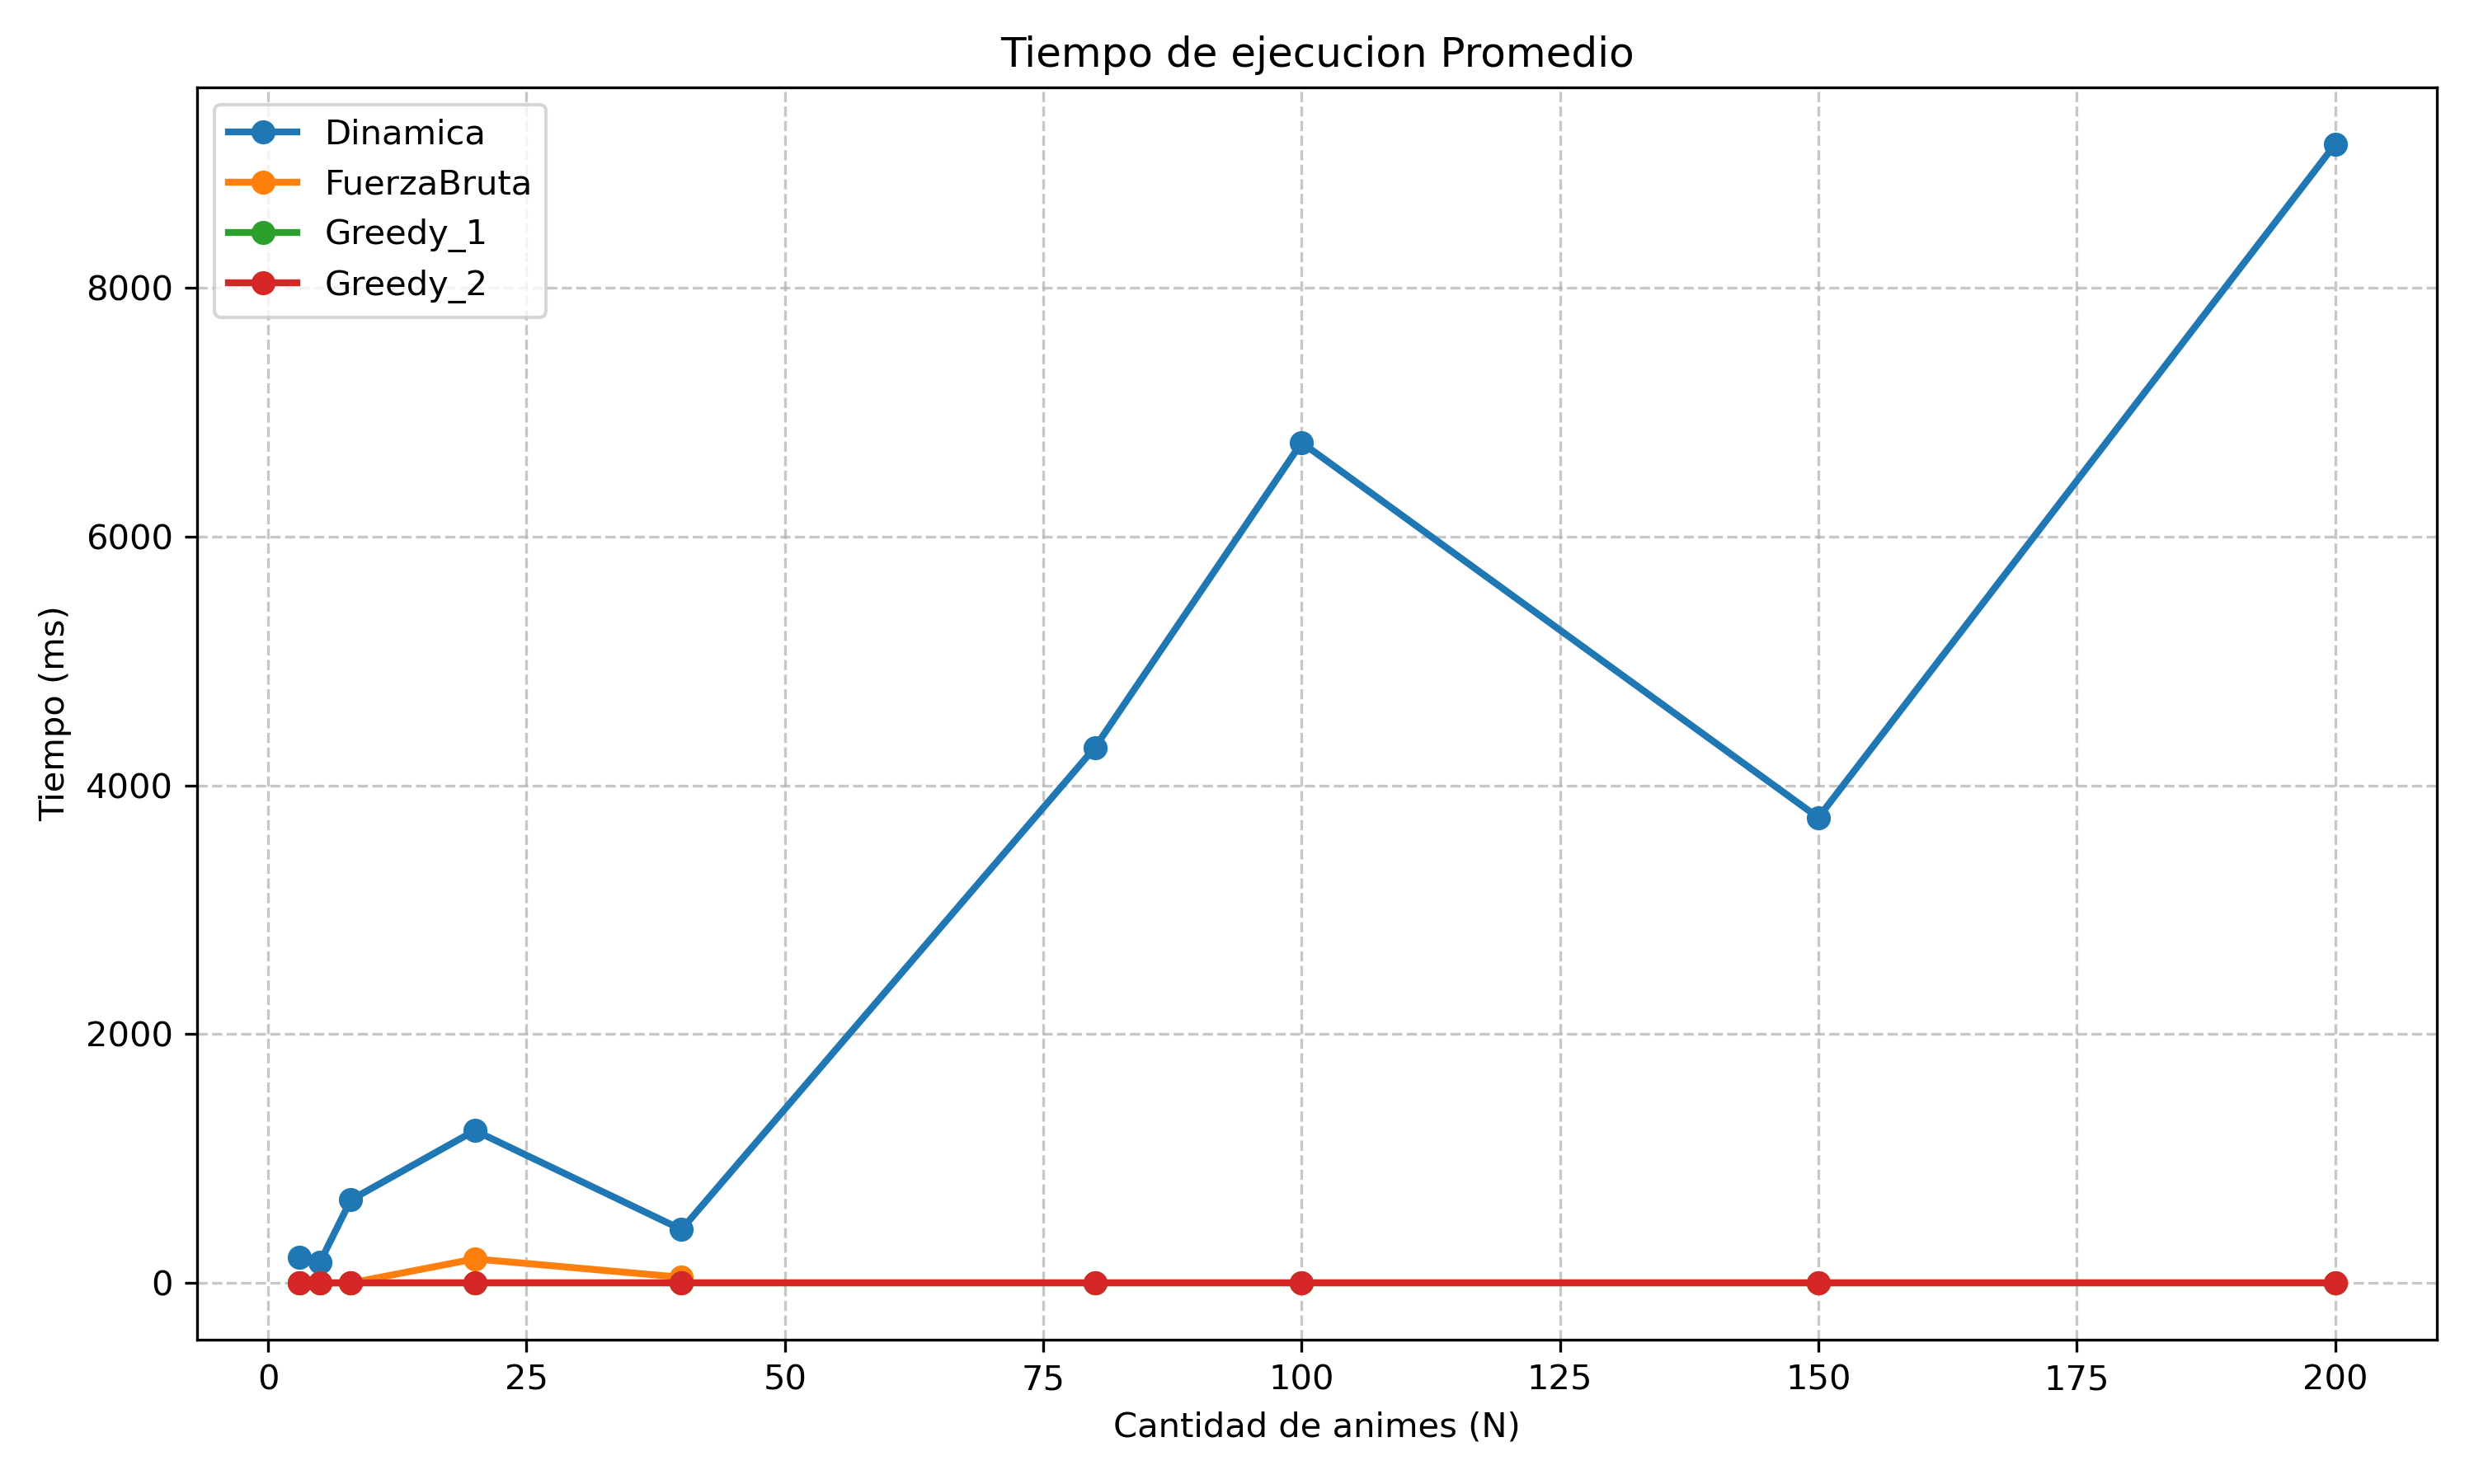
\includegraphics[width=\textwidth]{../code/implementation/data/plots/tiempo_ejecucion.png}
    \end{minipage}%
    \begin{minipage}[t]{0.5\textwidth}
        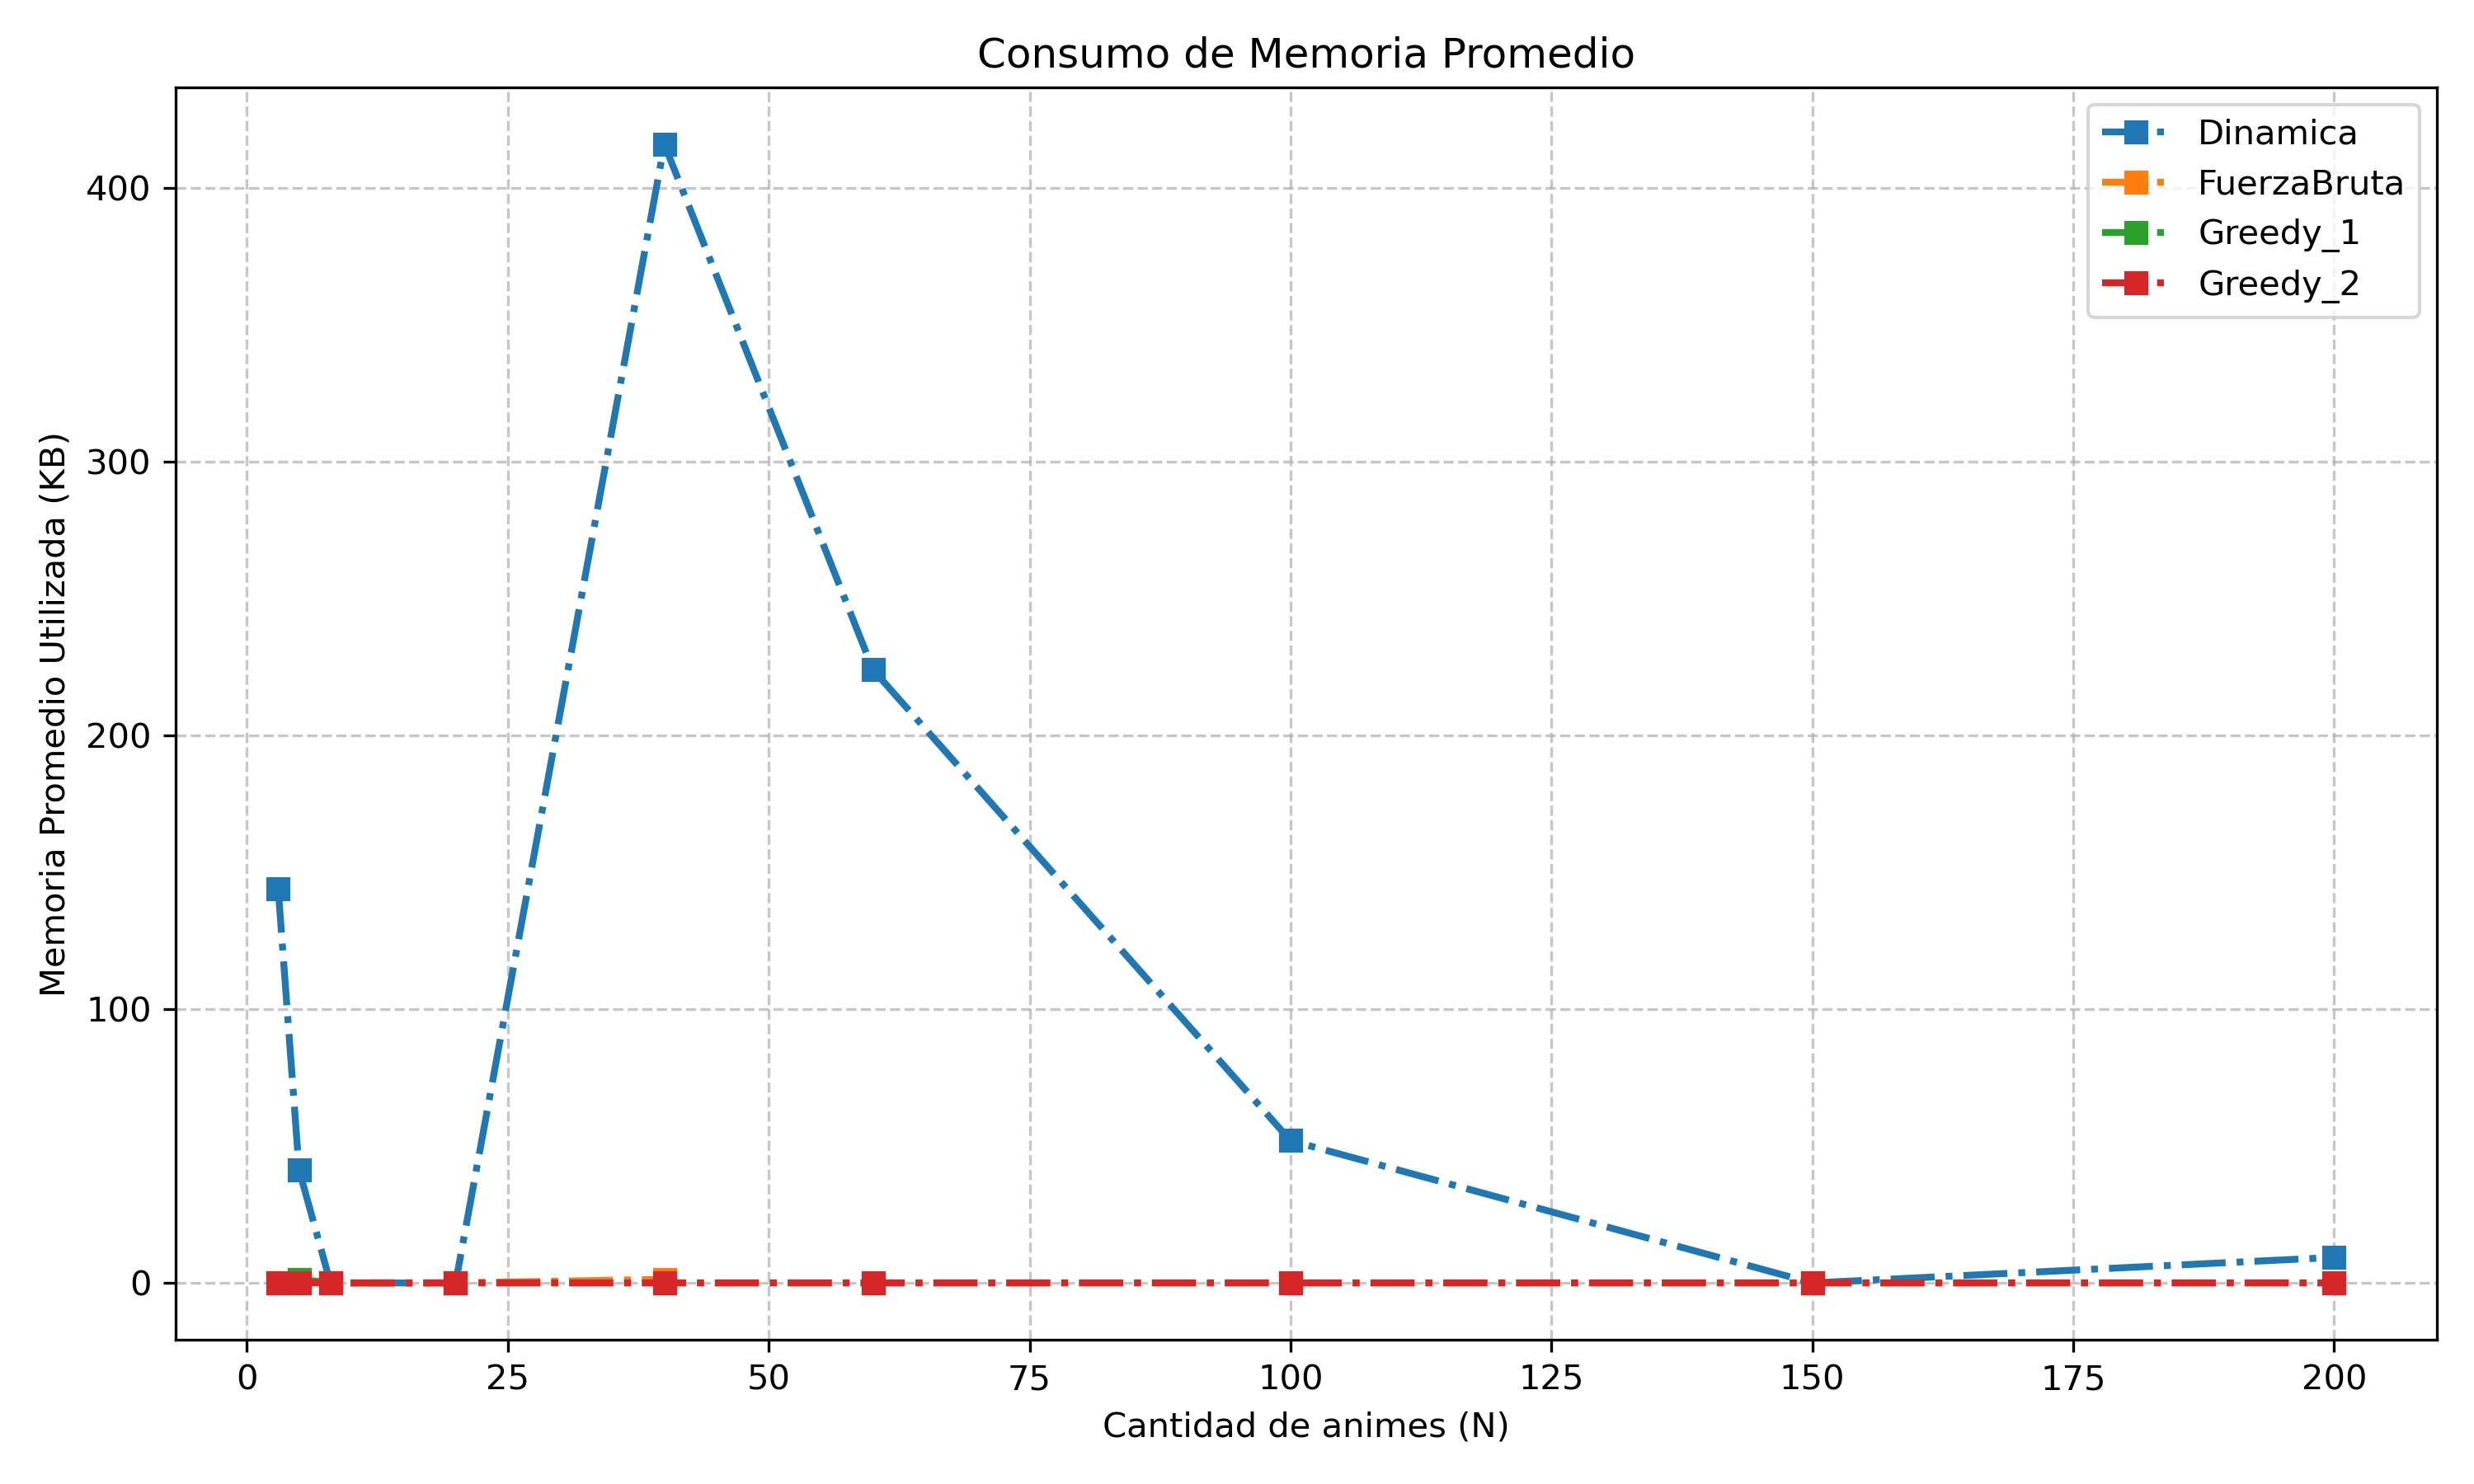
\includegraphics[width=\textwidth]{../code/implementation/data/plots/consumo_memoria.png}
    \end{minipage}%
    \caption{Comparación del tiempo de ejecución y consumo de memoria por cada algoritmo}
    \label{fig:grafico_tiempo_memoria}
\end{figure}

Como podemos observar, el algoritmo de programación dinámica presentó los tiempos y consumos de memoria más altos entre los 4 algoritmos (Al menos de lo que se aprecia de los gráficos, como fue dicho antes, fuerza bruta tomaba horas en casos n >= 60)
Y si bien hay una pequeña inconsistencia entre los n = 20 y n = 40, y entre n = 100 y n = 150 esto puede deberse a los atributos de tiempo y energía asignados por el generador de casos de prueba, pues se ha observado en las pruebas que eso puede llegar a influir.
Aun así, se aprecia a nivel general que entre mayor sea el n, mayor tiende a ser el tiempo de ejecución empleado.
\\


En el caso del algoritmo de fuerza bruta, hasta los tipos de casos en donde se probó, se observa cierto aumento en el tiempo de ejecución a medida que n crece (Salvo por el bajón que pega en n = 40, el cual puede deberse a la misma razón de la ''inconsistencia'' observada en programación dinámica.)
Y dado a lo mencionado en la nota, los casos de n > 60 tardaban horas, por lo que se decidió descartar finalmente de las pruebas empíricas, y limitandonos (por desgracia) a mencionar aquí que durante la realización de las pruebas (No llegando a la fase de medición y gráfico) fue el que evidentemente tardó más.
Algo que no se ha podido reflejar en los gráficos por la razón anteriormente mencionada.
\\

Además, en lo que respecta a los algoritmos de Greedy, estos presentaron tiempos relativamente bajos en todos los casos debido al enfoque de cada uno de ellos, sobre todo por evitar mayormente el uso de ciclos anidados en su estructura algorítmica, lo cual influyó en los bajos tiempos obtenidos.
\\

En cuanto al uso de memoria, observamos que tanto fuerza bruta como las heurísticas de greedy no consumen casi nada de memoria dado al enfoque recursivo del primero, y el los enfoques específicos de las heurísticas.
Sin embargo, la programación dinámica presenta el mayor consumo de memoria al recurrir al uso de matrices para solucionar el problema de la satisfacción máxima, teniendo un pico máximo en n = 80. Ahora, también se puede observar una inconsistencia acá, pues se espera que los valores n mayores
tengan un mayor consumo de memoria, pero esto podría no ocurrir debido a como los casos de prueba han sido generados, con valores que podrían afectar en ello (aunque n = 200 presenta un ligero aumento en el consumo de memoria.).


Sin embargo ¿Los algoritmos Greedy ofrecen soluciones ''de calidad'' a pesar de tardar muy poco? Observemos los siguiente gráficos.


\textbf{Comparación de calidad de solución entre greedy y programación dinámica.}


Para ello hemos de compararlo con el enfoque de programación dinámica, puesto a que este nos entrega la satisfacción más precisa para cada caso de prueba frente a los otros enfoques.


Al comparar las heurísticas de greedy con la programación dinámica obtenemos lo siguiente:

\begin{figure}[H]
    \centering
    \begin{minipage}[t]{0.5\textwidth}
        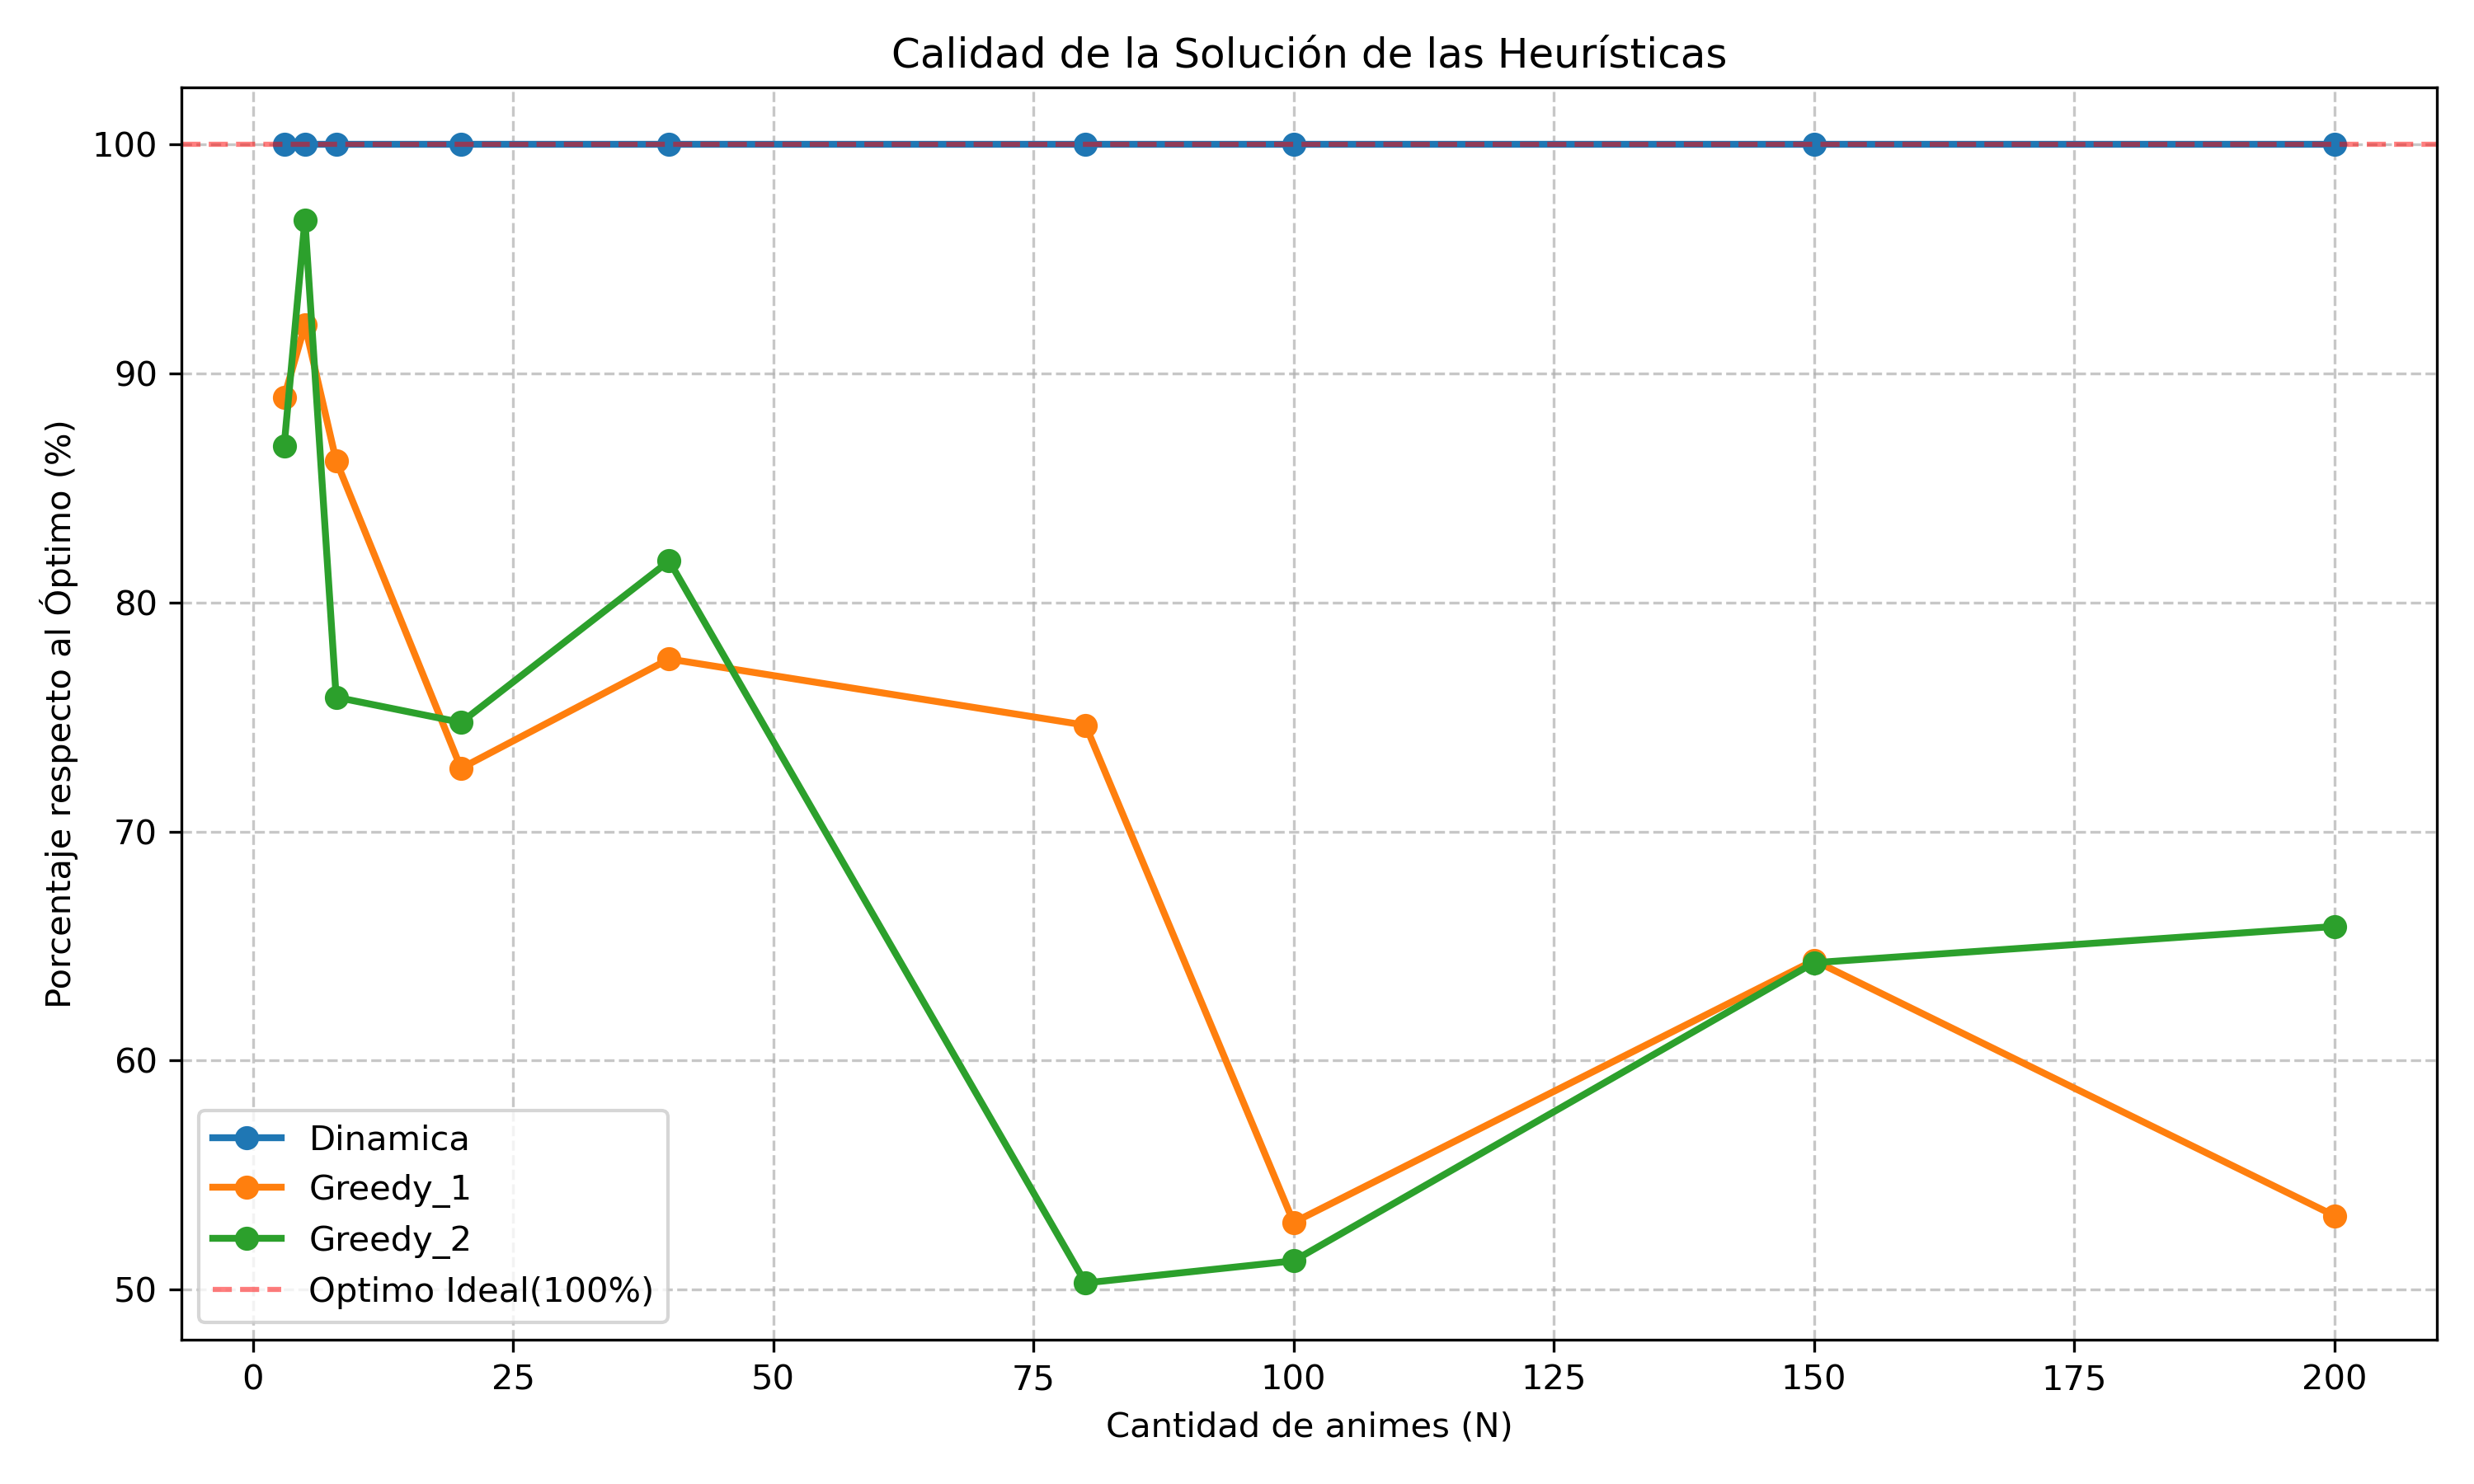
\includegraphics[width=\textwidth]{../code/implementation/data/plots/calidad_solucion.png}
    \end{minipage}%
    \caption{Comparación de la calidad de solucion entre greedy y programacion dinamica}
    \label{fig:grafico_tiempo_memoria}
\end{figure}

Como se puede apreciar, a nivel general la segunda heurística presenta resultados más cercanos al resultado esperado en los n > 80.
Sin embargo, observamos que en los valores más ''intermedios'' la primera heurística presenta mejores resultados hasta n = 100, y finalmente en casos
Donde n = 150 ambos presentan la misma calidad pero en n = 200 la primera heurística cae bastante mientras que la segunda ofrece un mejor resultado en este aspecto.
\\

También es fácil notar que a medida que n aumenta la calidad de las soluciones decae, logran recuperarse un poco y al final una de ellas destaca un poco más.
\\

Con ello, observamos que estas heurísticas implementadas si bien presentan soluciones más rápidas al problema de este experimento, estas son más efectivas para valores n pequeño, y ya en n más grandes ofrecen resultados no tan confiables
comparado con la programación dinámica, por lo que una solución más rápida no necesariamente ofrece los resultados más precisos ni confiables y pueden variar dependiendo de varios factores en cómo están hechos los casos de prueba, así como el tamaño n de estos mismos.
